%%portail-ajout-application.tex
\section{Ajouter une application au profil}
Cette fois-ci c'est l'onglet \bsc{application} qui devra être sélectionnée.
\begin{figure}
	\centering
	
\includegraphics[width=\linewidth]{./Captures/portail.barre.seule.png}
%	\caption{}
\end{figure}
Dès lors, la liste des applications disponible apparaît avec des icônes permettant de filtrer par centre d'intérêt.
\begin{figure}
	\centering
	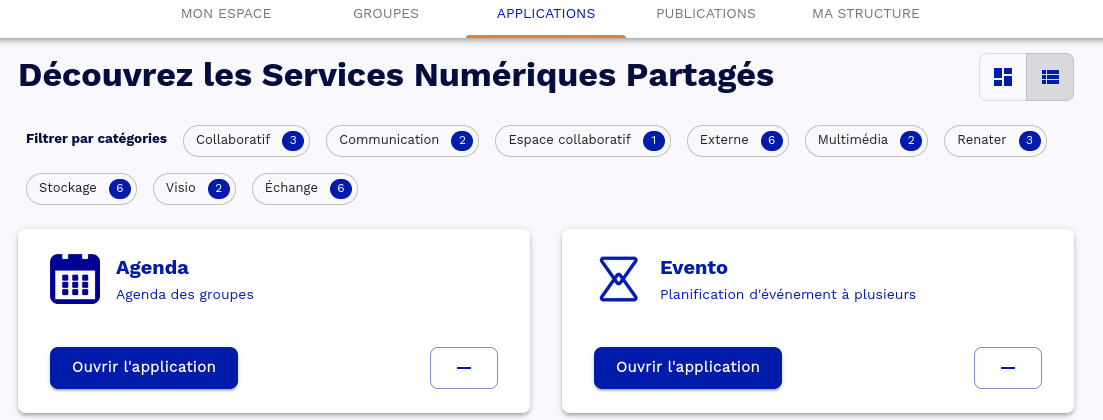
\includegraphics{./Captures/portail.applications.selection.png}
	\caption{sélectionner des applications}
\end{figure}
La capture précédente montre que les deux applications, \textbf{Agenda} et \textbf{Evento} sont déjà ajoutées à mon profil car sinon l'icône en bas à droite serait un ``+'' pour l'ajouter, alors que là c'est un ``--'' qui est visible me permettant de retirer l'application du profil.
\begin{figure}
 	\centering
 	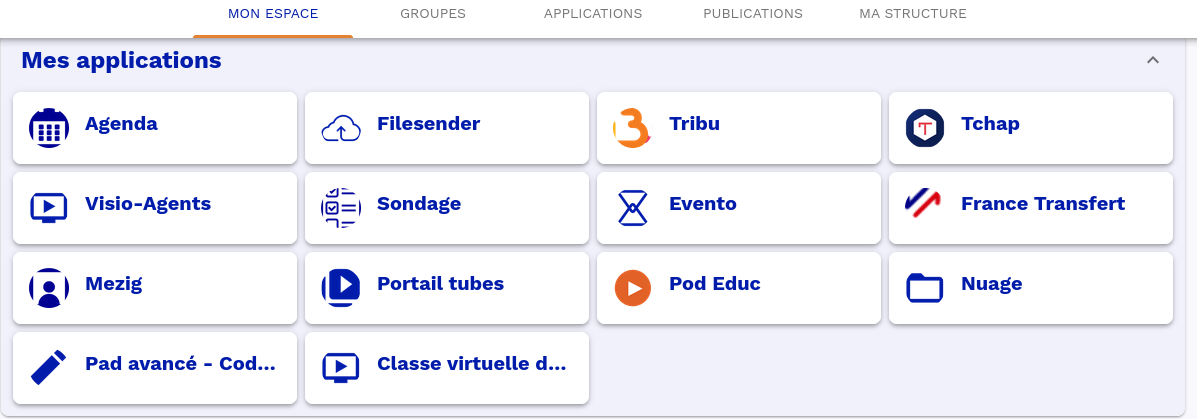
\includegraphics{./Captures/portail.mes.applications.png}
 	\caption{Les applications visibles et accessibles dans mon profil.}
 \end{figure}
Il est évidemment possible de retirer toute application du profil lorsque l'envie vous prendra.